


%!TEX TS-program = xelatex
%!TEX encoding = UTF-8 Unicode
%!BIB TS-program = biber
%!BIB program = biber
\documentclass[12pt,twoside]{book}
%\usepackage{extsizes}
\usepackage{geometry}                % See geometry.pdf to learn the layout options. There are lots.
\geometry{a4paper}                   % ... or a4paper or a5paper or ...
%\geometry{landscape}                % Activate for for rotated page geometry
%\usepackage[parfill]{parskip}    % Activate to begin paragraphs with an empty line rather than an indent section
\geometry{left=3cm}
\geometry{right=3cm}
\geometry{bottom=2cm}
\geometry{top=2cm}
\usepackage{graphicx}
\usepackage{amssymb}

\usepackage{polyglossia}
\usepackage[babel]{csquotes}
\setdefaultlanguage{german}

\usepackage{titlesec}
\usepackage{hyperref}
\usepackage[all]{hypcap} % Make references jump to the figure and not to the caption.
\usepackage{enumitem}

\usepackage{wasysym}
\usepackage{minted}

\usepackage{booktabs}
\usepackage{tabularx}

\usepackage{todonotes}

\usepackage{float}

\usepackage{tikz}

\usepackage{ifplatform}

\usepackage{savesym}
\savesymbol{iint}
\savesymbol{iiint}
\usepackage{amsmath}

\setlength{\parindent}{0cm}
\setlength{\parskip}{\medskipamount}

% Will Robertson's fontspec.sty can be used to simplify font choices.
% To experiment, open /Applications/Font Book to examine the fonts provided on Mac OS X,
% and change "Hoefler Text" to any of these choices.

\usepackage{fontspec,xltxtra,xunicode}

\ifmacosx
	\newcommand{\romanFont}{Hoefler Text}
\else
	\newcommand{\romanFont}{Linux Libertine O}
\fi

\defaultfontfeatures{Mapping=tex-text}
\setmainfont[Mapping=tex-text]{\romanFont}
%\setsansfont[Scale=MatchLowercase,Mapping=tex-text]{Gill Sans}
%\setmonofont[Scale=MatchLowercase]{Andale Mono}
% \setmonofont[Mapping=tex-text,%
%     ItalicFont=Source Code Pro ExtraLight,%
%     BoldFont=Source Code Pro]{Source Code Pro Light}

%\newcommand{\HRule}{\rule{\linewidth}{0.1pt}}
%\newcommand{\logoheight}{2.5cm}

\renewcommand{\title}{DAI Infoboard}
\renewcommand{\author}{Tom Nick}
%\date{}                                           % Activate to display a given date or no date

% PDF properties
\hypersetup{
	pdftitle={\title{}},
	pdfauthor={\author{}}
}

\usepackage[style=authoryear,natbib=true,backend=biber]{biblatex}
\bibliography{bachelorthesis}{}

\setlength{\bibitemsep}{8pt}
%\setlength{\bibhang}{0.2cm}

\usepackage{xpatch}
\xpretobibmacro{author}{\mkbibbold\bgroup}{}{}
\xapptobibmacro{author}{\egroup}{}{}
\xpretobibmacro{bbx:editor}{\mkbibbold\bgroup}{}{}
\xapptobibmacro{bbx:editor}{\egroup}{}{}

\renewcommand*{\labelnamepunct}{\mkbibbold{\addcolon\space}}


\usepackage{changepage}

\makeatletter
\renewcommand\listoffigures{%
    \section*{\listfigurename}% Used to be \section**{\listfigurename}
      \@mkboth{\MakeUppercase\listfigurename}%
              {\MakeUppercase\listfigurename}%
    \@starttoc{lof}%
    }
\makeatother

\makeatletter
\renewcommand{\todo}[2][]{\tikzexternaldisable\@todo[#1]{#2}\tikzexternalenable}
\makeatother

\setcounter{secnumdepth}{3}
\setcounter{tocdepth}{2}

%\newcommand*{\fullref}[1]{\hyperref[{#1}]{\autoref*{#1} \nameref*{#1}}}
\newcommand*{\fullref}[1]{\hyperref[{#1}]{\autoref*{#1} (\nameref*{#1})}}

\newcommand{\makemu}{{\fontspec{Linux Libertine O}μ}}

\usepackage{multirow}

\usepackage{capt-of}

\usepackage[hang,flushmargin,bottom]{footmisc}

\newenvironment{absolutelynopagebreak}
  {\par\nobreak\vfil\penalty0\vfilneg
   \vtop\bgroup}
  {\par\xdef\tpd{\the\prevdepth}\egroup
   \prevdepth=\tpd}

\usepackage{titlesec}

\titleformat{\chapter}[display]
    {\normalfont\huge\bfseries}{\chaptertitlename\ \thechapter}{20pt}{\Huge}
\titlespacing*{\chapter}{0pt}{0pt}{40pt}

\usetikzlibrary{arrows,automata,positioning}

\usepackage{soul}

\usepackage{fancyhdr}
\fancyhead{}
\fancyfoot{}
\fancyhead[RE]{\textsc{\nouppercase{\rightmark}}}
\fancyhead[LO]{\textsc{\nouppercase{\leftmark}}}

\fancyfoot[CO,CE]{\thepage}
\pagestyle{fancy}

\setlength{\headheight}{14.5pt}

\let\cleardoublepage\clearpage

\usepackage[section]{placeins}

\usepackage{afterpage}
\newcommand\blankpage{%
    \null
    \thispagestyle{empty}%
    \addtocounter{page}{-1}%
    \newpage}

\usepackage{listings}



\begin{document}

% Titlepage
\begin{titlepage}
%\includegraphics[height=\logoheight,page=1]{Telekom_Logo_bw.pdf} \hfill \includegraphics[height=\logoheight,page=1]{TU_Logo.pdf}
\begin{center}
%\vspace{1cm}
%{\Huge Bachelor}\\
{\Huge \textsc{Technische Universität Berlin}}
{\fontsize{2.5cm}{2cm}\selectfont \textsc{Bachelor Thesis}\par}
\vspace{1cm}
\hrule
\vspace{0.3cm}
{\Huge \textsc{\title{Enterprise Infoboard - Intelligente Visualisierung und Austausch von heterogenen Informationen im Unternehmen}}\par}
~\\[0.1cm]
{\Large Supervisor: Prof. Albayrak}\\[0.1cm]
{\Large Advisors: -}\\[0.3cm]
{\Large Written by \author{}}\\[0.1cm]
{\Large \today}
\vspace{0.55cm}
\hrule
\end{center}
%\vspace{1cm}
\vfill
\begin{center}{\Large\textbf{Abstract}}\end{center}

Das DAI-Labor ist ein Innovationsleiter in Sachen verteiltee Suchmaschinen - welche nun nicht mehr reine Forschung sind, sondern wie deren PIA-System von vielen Verwaltungen als Alternative zu privaten Suchmaschinen benutzt wird. Einer der Kernherrausforderungen bei Suchmaschinen mit vielen komplett seperaten Suchindizes ist es die Ergebnisse dieser zusammen zu führen und für den Endbenutzer zu visualiesieren. Diese Arbeit zielt darauf ab eine Visualisierungsform die ähnlich zu einer \textit{social media wall} sein soll für diese Ergebnisse zu untersuchen und zu erstellen. Desweiteren werden kollabaritive Elemente untersucht d.h. Ergebnisse mehrerer Benutzer werden gleichzeitig angezeigt und eine Anzeige vergleichbar mit der \textit{frontpage} von reddit, wo die Suchergebnisse aller Benutzer angezeigt werden. Das Ergebnis ist eine voll funktionsfähige Webapplikation die neben der reinen Visualisierung und Interaktion der Elemente,\textit{Gamification} benutzt um die (kollabaritive) Nutzung zu fördern indem Benutzer \textit{belohnt} werden für die Benutzung sowie dafür das andere Benutzer ihre Inhalte \textit{gut} finden.

\end{titlepage}

\pagenumbering{roman}

%\blankpage

\chapter*{Declaration of authorship}

I hereby certify that the thesis I am submitting is entirely my own original work except where otherwise indicated. I am aware of the University's regulations concerning plagiarism, including those regulations concerning disciplinary actions that may result from plagiarism. Any use of the works of any other author, in any form, is properly acknowledged at their point of use.\footnote{The template for this declaration of authorship was taken from \url{https://www.wiwi.hu-berlin.de/international/mems/upload/authorship}.}

\vspace{2cm}

Berlin, \today\\
\textbf{Place, date}\hfill\textbf{Signature}

\tableofcontents
\newpage

\pagenumbering{arabic}

\chapter{Einleitung}

\section*{Motivation}

Die gemeinsame Darstellung von Inhalten verschiedener Quellen ist ein interessantes und weit erforschtes Thema. Die grundsätzliche Idee ist dem Benutzer die Benutzung bzw. die Konsumierung von Inhalten angenehmer zu gestalten indem ein einheitliches Interface für Inhalte geschaffen wird. Bevor der \textit{digitalen Revolution} war dies ein immens aufwendiges und kostpieliges Unterfangen, als Beispiel sei die frühen Enzyklopädien genannt\footnote{Enzyklopädien sind insofern eine einheitliche Aggregierung des Inhalts, das sie versucht haben sämtliches Wissen in einer Quelle bereitzustellen die homogen in Sprache und Darstellung ist.}. Durch die momentan verfügbaren Technologien ist das erstellen einer einheitlichen Datenquelle für verschiedene Inhalte deutlich einfacher geworden, wobei die Schwierigkeit einer guten zusammenführung dennoch weiterhin besteht und Produkte die dies gut machen sehr erfolgreich sind - wie z.B. die Suchmaschine von Google.
Wenn man sich jedoch auf eine Teilmenge der verfügbaren Informationen beschränkt wie z.B. Nachrichten die per RSS\footnote{Ein weit verbreitetes Dateiformat im Internet \url{http://de.wikipedia.org/wiki/RSS}} verfügbar sind ist es deutlich einfacher eine angemessene zusammenführung der Inhalte zu gestalten, prominente Beispiele für eine Anwendung dieser Art ist z.B. die Nachrichten-Applikation \textit{pulse}\footnote{\url{https://www.pulse.me/}} die auf Basis von RSS ein angenehmens und sehr attraktives Interface für die gleichzeitige Konsumierung mehrerer Nachrichtenseiten anbietet, der Erfolg von \textit{pulse} spricht für sich\footnote{ca. 22 Millionen Downloads auf dem Android-System}. Diese Arbeit zielt auf einen Spezialfall der Darstellungsformen verschiedener Inhalte ab, die der \textit{social media wall} was eine populäre Form für Inhalte mit kurzen Texten und oder Bildern ist\footnote{Natürlich sind auch Inhalte anderer Art möglich, jedoch sind die Elemente solcher Wände in jeglichem Aspekt daraufhin optimiert.}.

Gamification hat in den letzten Jahren stetig an Zuwachs gewonnen da es ein äußerst effektives Mittel ist um Benutzer zu binden, was bei der immer größer werdenden Konkurrenz bei digitalen Produkten immer schwerer wird. Die Benutzung von Gamification im Enterprise-Bereich bzw. in kleinen sozialen Kreises ist jedoch bisher noch nicht allzu populär, die prominentesten Beispiele sind Sport-Apps bei denen Freunde sich miteinander vergleichen können. Eine Integration von Gamification stellt damit in diesemen Bereich eine interessante Herausforderung da, dessen Potential bisher noch nicht geklärt ist.


\section*{Anforderungen}

Die Anforderungen der Applikation waren von vornerein nicht vollständig geklärt, viel mehr gab es ein grobes Gerüst was die Anwendung liefern sollte. Die komplette Ausarbeitung ist während der Entwicklung geschehen.

\subsection*{Darstellung von Daten}

  Einer der Hauptanforderungen ist die Darstellung von Datenpunkten (im zukünftigen Verlauf des Textes wird die Darstellung dieser Datenpunkte als \textit{Kacheln} bezeichnet) im Stil einer \textit{Social Media Wall}. Daraus folgen weiterhin die Anforderungen dass es unterschiedliche \textit{Kacheln} gibt - also für verschiedene Daten verschiedene Darstellungen z.B. könnten Suchergebnisse für Kontakte und Webseiten ganz unterschiedlich aufgebaut sein. Die dargestellten Inhalte sind weiterhin dynamisch, während des Betriebes können Kacheln hinzukommen/entfert werden und auch die Interaktion mit den Kacheln kann das Layout ändern.

\subsection*{Bewertungssystem}

  Der Benutzer soll in der Lage sein angezeigte Suchergebnisse zu bewerten und dadurch zukünftige Anfragen für \textbf{alle} Benutzer zu verändern.

\subsection*{Benutzung mehrerer Datenquellen}
  Die angezeigten Daten können aus mehreren Datenuellen kommen, d.h. die gleichzeitige Darstellung von Daten von z.B. Facebook mit denen von Twitter. Hier war es wieder besonders wichtig, dass man einfach neue Datenquellen hinzufügen kann. Auch das während des Betriebes vorhandene Quellen mit anderen Parametern (wie einer Suchanfrage) neu hinzugefügt werden kann.

\subsection*{Authentifizierungssystem}
  Das DAI stellt aus gutem Grund ihre Datenquellen nur intern zu Verfügung bzw. nur nach einer Authentizieferung mittels Benutzername/Passwort, somit muss die Applikation in der Lage sein diese Authentfizierung auszuführen und sicherzustellen dass niemals \textit{zuviel} unauthentifizierten Benutzern angezeigt wird.

\subsection*{Single Page Application}
  Es soll eine sogenannte \textit{Single Page Application} werden, d.h. eine Webapplikation bei der JavaScript abseits des initialen Seitenaufrufes alles rendert, im Gegensatz zur klassischen Methodik bei der jede Interaktion zu einer komplett neuen Seite die vom Server gerendert wird resultiert.

\subsection*{Gamification}
  Um die Benutzung der Seite zu animieren sollen Gamification-Methoden eingeführt werden wie z.B. Punkte für das tägliche einloggen bis hinzu erweiterten Methoden wie eines Compulsion Loop.

\subsection*{Konfiguration}
  Es muss möglich sein viele Parameter anzupassen, einige davon auch als Benutzerinterface für den Benutzer andere wiederum als simple Konfigurationsdatei für verwendete URLs und ähnliches.

\section*{Relevante Arbeiten}

Da die Applikation mehrere Gebiete vereint als etwas bestehendes weiterzuentwickeln, gibt es direkt keine relevanten Arbeiten. Jedoch ist es nützlich bestehendes in den einzelnen Gebieten zu untersuchen.

\subsection*{Social Media Walls}

Eine sehr gute Auflisting verschiedener \textit{social media wall}-Applikationen bietet \citep{hofram}. Die Homogenität dieser Angebote ist erstaunlich, würde man die Produkte zweier verscheidener Anbieter nebeneinander sehen wäre der größte Unterschied kleinere stylistische Unterschiede wie benutzte Farben oder ähnliches. Leider sind die wenigsten Produkte in einer Demo zu testen, da die Lösungen meistens zugeschnitten werden für den Kunden, welcher diese meistens auf großen Veranstaltungen wie Konzerten verwendet. \\

\begin{figure}[H]
    \centering
    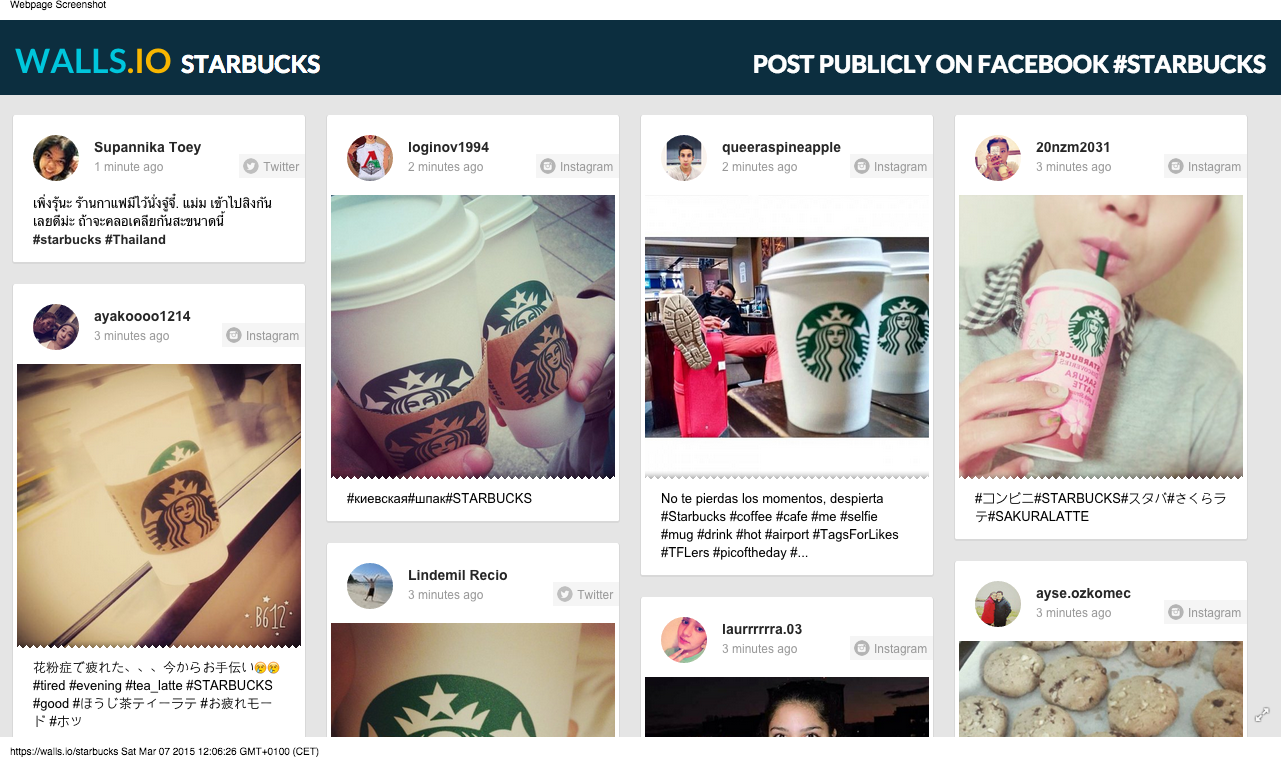
\includegraphics[width=0.8\textwidth]{images/Starbucks.png}
    \caption{Eine \textit{social media wall} vom Anbieter walls.io}
    \label{fig:awesome_image}
\end{figure}

Insofern sind diese Angebote für diese Arbeit nicht wirklich lohnenswert weiter zu analysieren und werden als grobe Inspiration für das Design benutzt.

\subsection* {Gamification}

Es gibt einige Seiten die ähnliche Inhalte anzeigen und erfolgreich Gamification implementiert haben. Einen sehr schwachen aber effektiven Ansatz verfolgt die Social-News-Seite \textit{reddit}\footnote{\url{http://reddit.com}}. Jegliche Inhalte (eingereichte Links, Kommentare) der Seite können binär bewertet werden (im reddit-jargon wird hier vom \textit{upvote} und \textit{downvote}) gesprochen. Reicht man nun selbst etwas ein, wird die Differenz aus \textit{upvotes} und \textit{downvotes} einem als \textit{Karma} gutgeschrieben. Jedoch besitzt Karma ähnlich wie die erreichte in Videospielen keinen Wert in dem Sinne, dass mit diesem nichts weiter gemacht werden kann als den Wert mit den von anderen zu vergleichen.
Dieser Gamification-Aspekt ist ein nicht zu unterschätzender Teil von \textit{reddit} bzw. dem Erfolg von \textit{reddit} welcher für sich spricht\footnote{laut Alexa ist \textit{reddit} die 29 meist besuchte Webseite der Welt, in den USA ist sie sogar Platz 10.}.
Eine ausführliche Untersuchung von \citep{richterichkarma} zeigt die Tragweite von \textit{reddits} Karma-System. Es dient demnach vorzüglich als Bewertung des eingereichten Inhalts durch andere bzw. die daraus resultierende Selbstbestätigung wenn das eigene Karma eröht wird.
Benutzer \textit{reddits} werden dadurch jedoch darauf gepolt ihre eingereichen Beiträge nach der Anzahl an Karma, welches der Beitrag liefern wird auszusuchen.

DAIKnow \citep{meder2014daiknow} ist eine Bookmarking Seite ähnlich zu \textit{delicous.com} bei der Links mit Beschreibungen und Keywords eingereicht werden können. Durch den gezielten Einsatz von Punkten, Trophäen und von Bestenlisten wird die Benutzung der Seite durch die Benutzer gesteigert. Im Gegensatz zu \textit{reddit} ist dieses System jedoch weitaus komplexer, so bekommet man z.B. Punkte für den täglichen Aufruf, Punkte für das einrechen eines Links oder das jemand anderes seinen Link kopiert hat.
Ein Problem das sich auftat bei DAIKnow war dass häufige Benutzer alle verfügbaren Trophäen freischalteten und damit der Gamification-Aspekt damit kein Grund mehr ist die Applikation weiter zu benutzen.

\chapter{Umsetzung}

\section*{Design}

Der wichtigste Aspekt für den Benutzer ist eine attraktive Darstellung und angenehme Bedienung der Applikation, natürlich neben dem Aspekt das es technisch an nichts mangelt d.h. es gibt keine Programmfehler und die nötigen Funktionen sind vorhanden. Im folgenden werden die einzelnen Aspekte der Darstellung dargestellt um die Findung der endgültigen Darstellung zu erklären.

\subsection*{Layout}

Wie \textit{social media walls} oder Websiten wie pinterest\footnote{\url{http://pinterest.com}} oder gar Microsoft mit ihrem metro-Design es gezeigt haben ist die aktuell beste Darstellung für Medieninhalte verschiedener Art ein Layout basierend auf Kacheln. Bei dem Anordnen gibt es verschiedene Ansätze:

\begin{itemize}
  \item \textbf{Spaltenbasierte Anordnung} \\
  Bei dieser Form werden die einzelnen Datenpunkte in Form von Kacheln mit einheitlicher Breite und variabler Höhe in Spalten in der Größenordnung von 3-5 dargestellt.

  \begin{figure}[H]
    \centering
    \includegraphics[width=0.5\textwidth]{images/livewall_columns.pdf}
    \caption{Spaltenbasierte Anordnung der Inhalte}
    \label{fig:awesome_image}
  \end{figure}

  \textbf{Vorteile} \\
  Die Vorteile liegen in der Simplizität der Implementierung und der Intuivität des \textit{content-flows} d.h. neuer Inhalt wird oben eingefügt und alter rutscht nach unten, wobei jeweils nur eine Spalte \textit{verrutscht} je neuem Datenpunkt.
  Weiterhin ermöglicht die Variable Höhe viel Flexibilität bei dem Anzeigen des Inhalts - z.B. könnten lange Texte angemessen gut angezeigt werden ohne die Zeichenanzahl zu limitieren oder ähnliches.

  \textbf{Nachteile}\\
  Der Größteile Nachteil ist die starre des Layouts, da alle Objekte die gleiche Breite haben ist man stark limitiert wie man die Inhalte darstellt.

  \item \textbf{Rasterbasierte Anordnung}
  Bei dieser Form werden die einzelnen Datenpunkte in einem einheitlichen Raster dargestellet, d.h. die darstellende Fläche wird in einem Raster der Größe $(a, b)$ unterteilt, die Kacheln können nun die Größe $(x, y)$ mit $ x \in \{1, \dots, a, y \in 1, \dots, b$ besitzen.

  \begin{figure}[H]
    \centering
    \includegraphics[width=0.8\textwidth]{images/livewall_grid.pdf}
    \caption{links: Das Raster des Grids, rechts: eine zufällige Benutzung des Grids}
    \label{fig:awesome_image}
  \end{figure}

  \textbf{Vorteile} \\
  \begin{itemize}
    \item Ansprechendes Aussehen
    \item Wichtigkeit kann durch größe der Kachel dargestellt werden
    \item Unterschiede in der Darstellung gleicher Datenpunkte durch unterschiedliche Größe
    \item Vorteilhaft bei der Anzeige ohne Interaktion, da es keine abgeschnittenen Inhalte gibt wie bei dem Spaltendesign
  \end{itemize}

  \textbf{Nachteile}\\
  \begin{itemize}
    \item komplexes flow-Verhalten bei neuem Inhalt
    \item Es müssen komplexere Methoden benutzt werden um Löcher zu verhindern
    \item Es müssen Design für die verschiedenen Kachelgrößen erstellt werden
    \item unterschiedliche Darstellungsformen können unübersichtlich wirken
  \end{itemize}

  \subsection*{Probleme beim Flow-Verhalten}
  Das Flow-Verhalten beim einfügen neuer Inhalte ist bei einem grid-basierten Layout mit unterschiedlichen Kachelgrößen äußerst komplex, im ersten Schritt müsste das Behälterproblem\footnote{} gelöst werden und im zweiten Schritt müssten die Elemente mittels anhand ihrer Bewertung nochmals sortiert werden. Die Lösungen des Behälterproblem darauf hin zu optimieren das der optische Fluss der Elemente minimiert wird scheint mir eine nicht einfache Aufgabe zu sein, weshalb man sich mit den \textit{schlechten} Lösungen zufrieden geben muss. Die JavaScript-Bibliothek \textit{packery} implementiert den ersten Schritt und ordnet die Element anhand einer Lösung des Behälterproblems, bei deren \textit{prepend}-Methode kann sehr gut erahnt werden wie \textit{wild} der Fluss bei jedem neuen Element wäre\footnote{\url{http://packery.metafizzy.co/methods.html\#prepended}}.

  \begin{figure}[H]
    \centering
    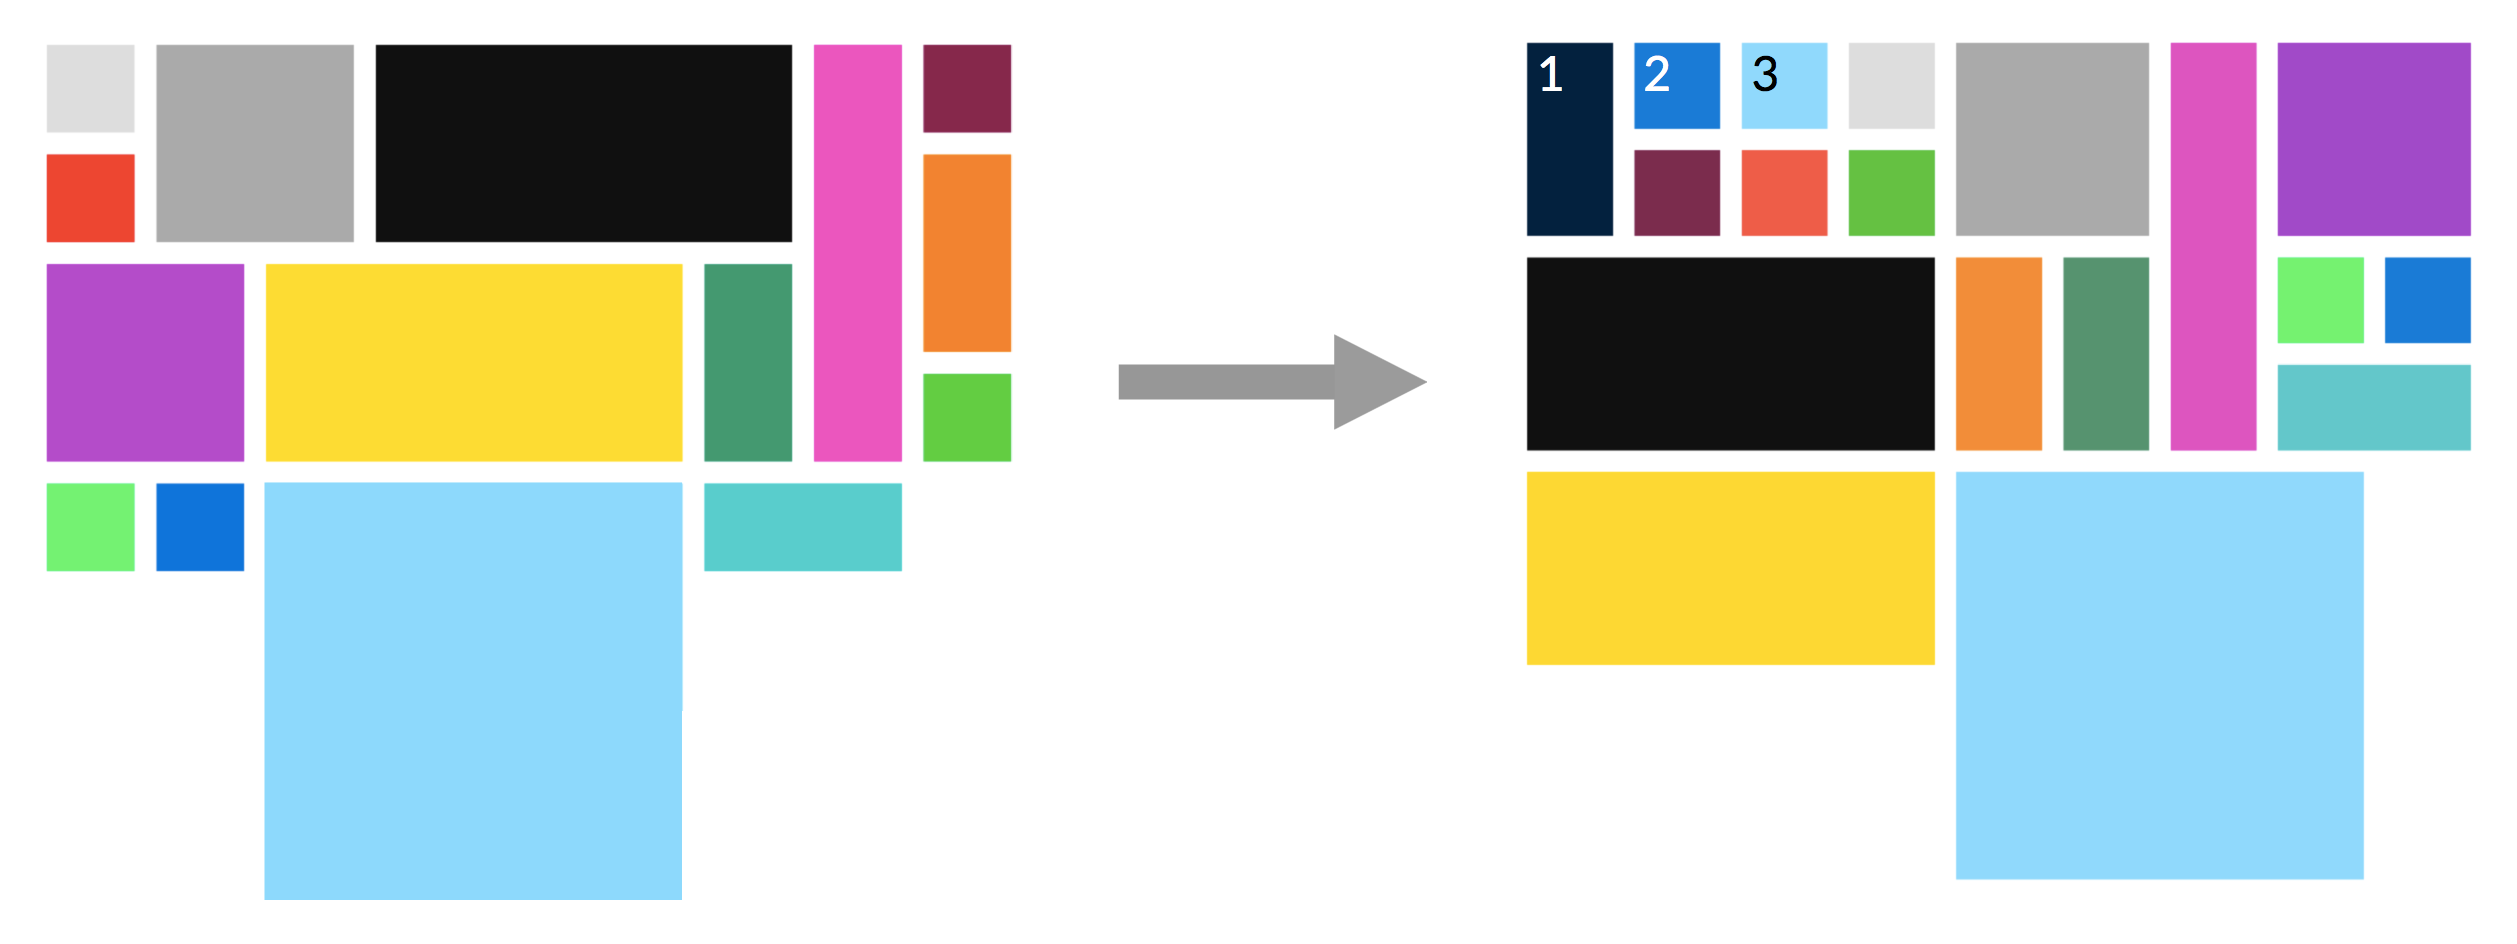
\includegraphics[width=0.8\textwidth]{images/grid_flow.png}
    \caption{Zu dem Grid links wurden die Elemente 1, 2 und 3 hinzugefügt. Das resultierende neue Layout ist rechts zu sehen. Dies ist ein praktisches Beispiel welches mithilfe von packery gemacht wurde.}
    \label{fig:awesome_image}
  \end{figure}


\end{itemize}

\subsection*{Animationen}

Eines meiner Ziele waren Animationen die neben dem rein ästhetischen Aspekt einen Vorteil im Verständnis des Datenflusses der Applikation ermöglicht.

\begin{enumerate}
  \item Neue Kacheln sollen von \textit{oben} kommen um einerseits zu zeigen dass es neue Inhalte gibt und andererseits um das vertraute Konzept zu benutzen dass neue Dinge meistens von oben kommen\footnote{Siehe z.B. Börsenticker, Nachrichtenseiten oder die Abfahrttafeln am Bahnhöfen} und nicht überraschend irgendwo auftauchen.\footnote{Vergleich zu Googles Material Design bei dem sehr viel Wert darauf gelegt wird sinnvolle Animationen zu machen, die den Benutzer unterstützen und nicht verwirren}
  \item Die neuen Kacheln ordnen sich an ihrem Platz ein (ein Algorithmus benutzt verschiedene Werte um das zu bestimmen), alte Kacheln machen dementsprechend Platz.
  \item Die Anzahl an Bewegungen soll minimal sein um nicht unnötig vom eigentlichen Inhalt abzulenken.
\end{enumerate}

Nur das Spaltenbasierte Layout erfüllt diese Anforderungen für Animationen, da der \textit{reflow} bei dem Kachelbasierten zu aufwändig ist, als dass nachverfolgt werden kann wie die Kacheln sich bewegen und welchen Gesetzenmässigkeiten sie unterliegen.

\subsection*{Kacheln}

Das Design der Kacheln ist neben derer Anordnung die wichtigste Design-Entscheidung. Neben dem rein funktionalen Aspekt ist auch das Aussehen wichtig um z.B. die einzelnen Inhalte gut voneinander zu unterscheiden und den Benutzer nicht zu überfordern.

Rein funktional besitzt eine Kachel folgende Anforderung:

\begin{itemize}
  \item Anzeige des gefundenen Inhalts und Möglichkeit diesen zu öffnen. Die Anzeige des Inhalts kann variieren.
  \item Benutzer können den Inhalt favorisieren (speichern) und bewerten.
  \item Es werden Metainformationen wie der Typ des Inhalts (PDF, Kontakt, ...) angezeigt.
  \item Kacheln können schnell zu dem Suchbegriff zugeordnet werden von dem Sie stammen.
\end{itemize}

Obwohl die Kacheln je nach dargestellten Inhalt stark variieren können ist es ratsam ein einheitliches Benutzerinterface für die Benutzerinteraktionen zu bieten. Auch sollten die Metainformationen gleich angezeigt werden.
Mit diesen Anforderungen kann eine funktionale Kachel konzipiert wie unten konzipiert werden.

\begin{figure}[H]
    \centering
    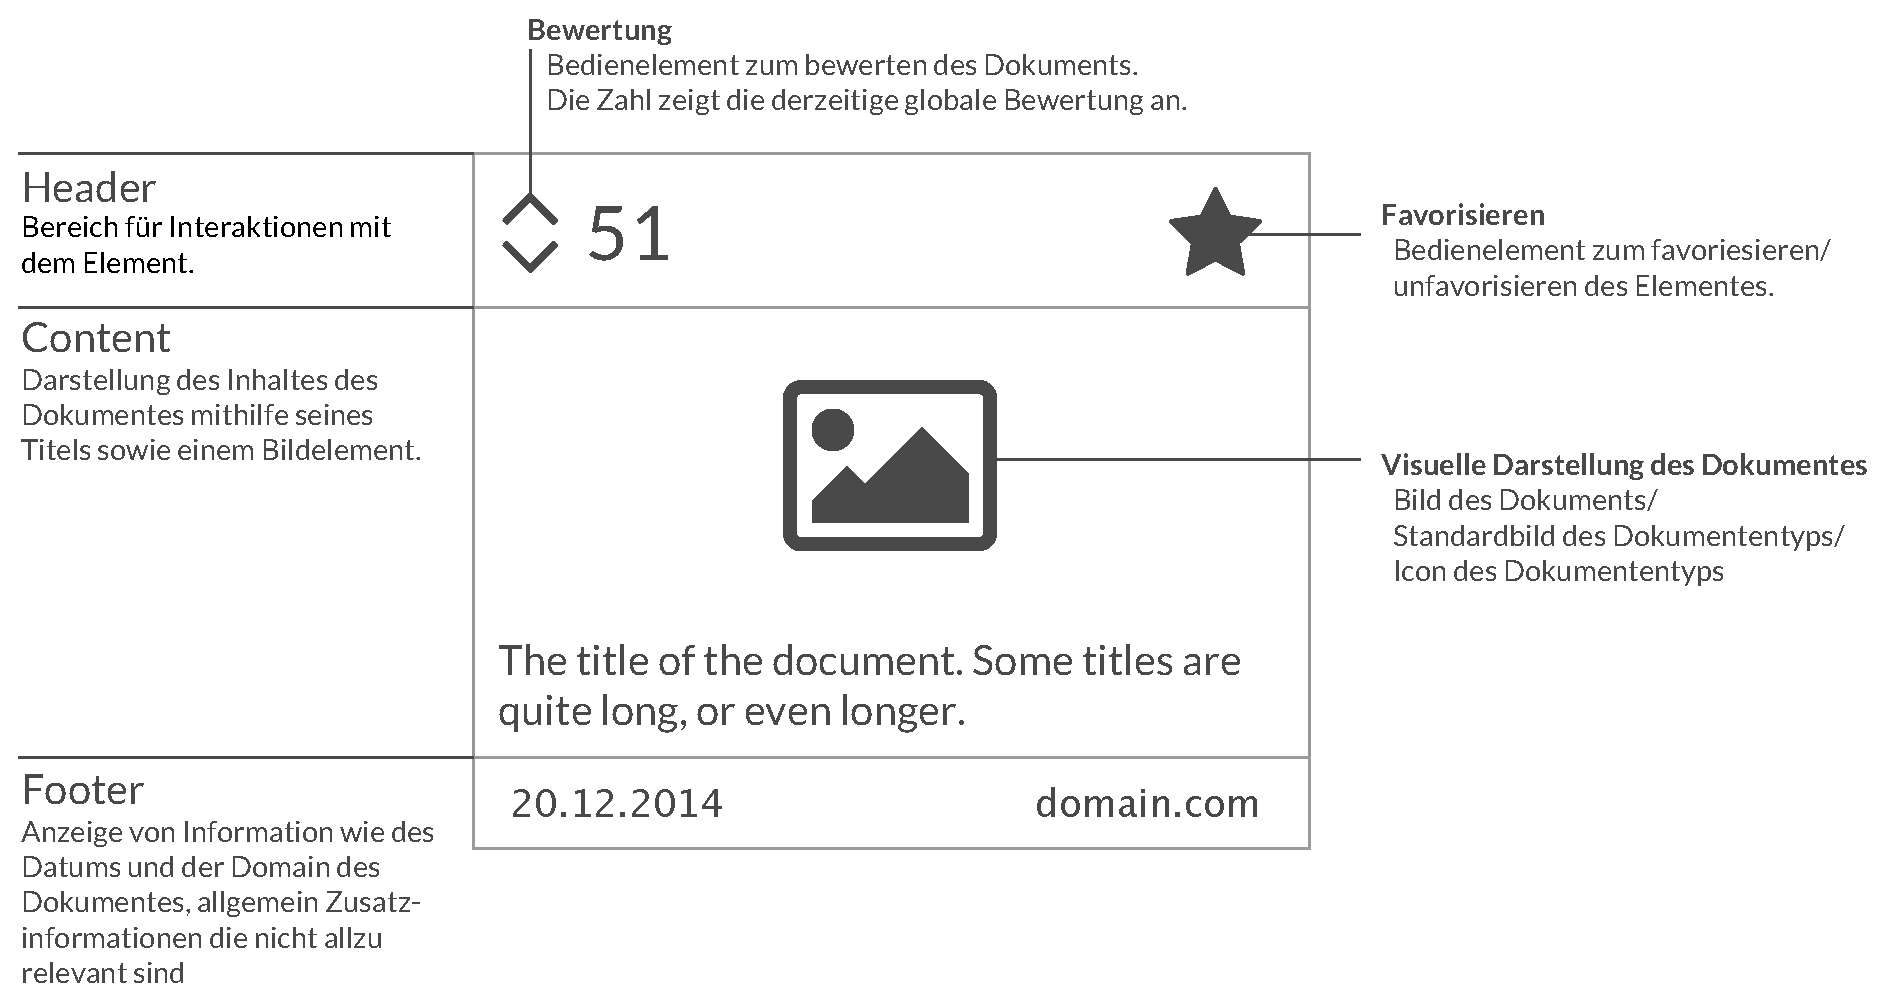
\includegraphics[width=1.0\textwidth]{images/tiles.eps}
    \caption{Eine prototyp-Kachel mit rein funktionalen Aspekten.}
    \label{fig:awesome_image}
\end{figure}

Menschen sind äußerst gut darin Farben und unterschiedliche Formen schnell zu gruppieren, da nach aktuellem Kenntnisstand, dies Teile der ersten Verarbeitungsstufe von visuellen Informationen ist \citep{treisman1987merkmale}. Da für uns die schnelle Assoziation von Suchbegriff und Kachel äußerst wichtig ist, wurde die Hintergrundfarbe der Kachel dafür benutzt. Dies schränkt das Design aber insofern ein dass bis auf Grautöne und Abstufungen der verwendeten Hintergrundfarbe keine anderen Farben möglich sind (man könnte z.B. das Symbol zum Favorisieren nicht überall rot anzeigen), doch waren das dadurch erzielte Design so überzeugend, dass dies in Kauf genommen wurde.

\begin{figure}[H]
    \centering
    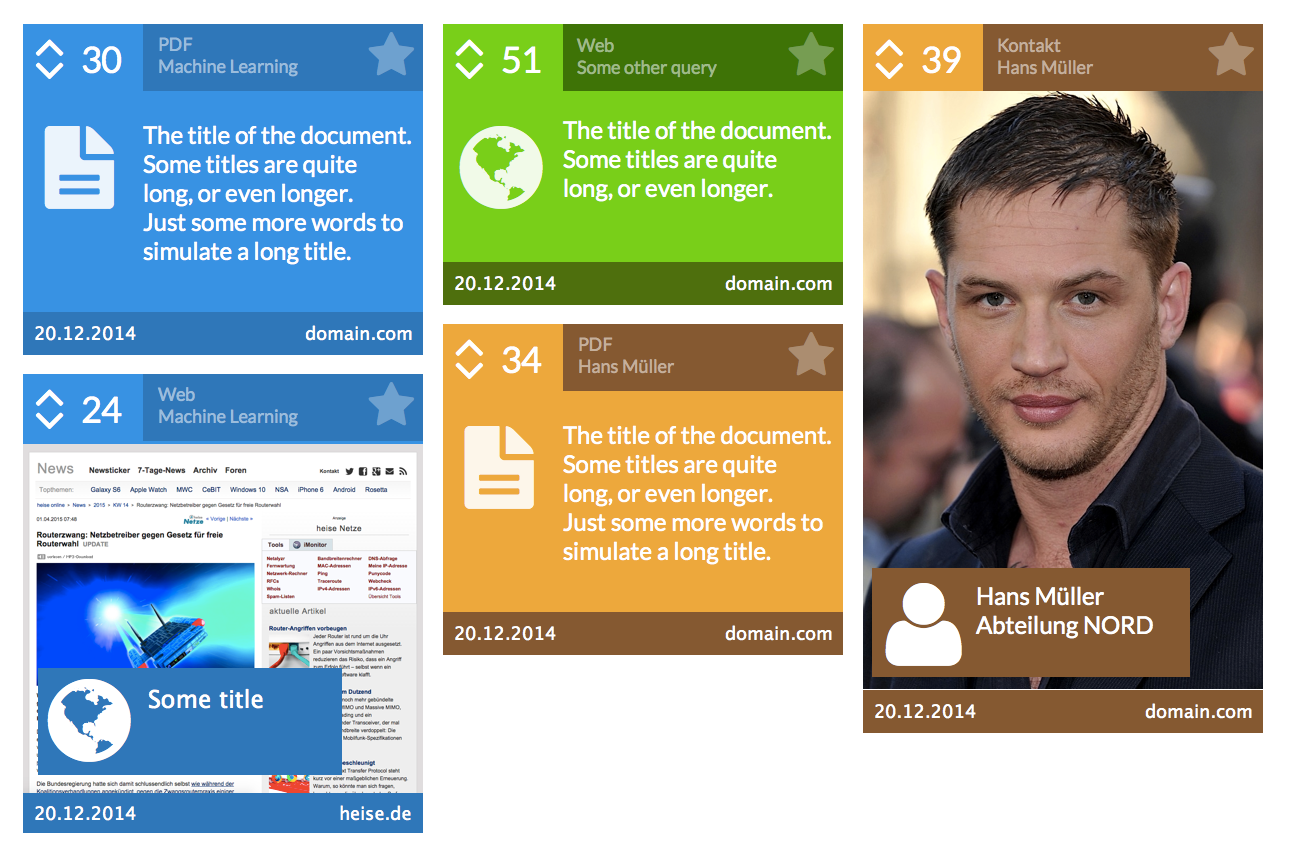
\includegraphics[width=1.0\textwidth]{images/tiles_real.eps}
    \caption{Ein erstes Design dass verschiedene Darstellungsformen für unterschiedliche Typen von Informationen benutzt.}
    \label{fig:awesome_image}
\end{figure}

\section{Gamification}

Wie sehr muss ich Gamification erklären?

Wie in der Einleitung erwähnt ist Gamification eine mittlerweile weitverbreitete und äußerst effektive Technik um Benutzer zu binden. Es ist schwer neue Technologien im Unternehmensfeld einzuführen, vor allem wenn sie freiwillig benutzt werden können - so wie das hier entwickelte Enterprise Dashboard. Ziel ist es also durch die Gamification der Benutzung die Benutzer dazu zu motivieren die Anwendung gewohnheitsmäßig zu benutzen.

Die Grundlage jeder verspielisierung ist der \textit{Compulsion Loop} welcher eine modellierte Kette an Aktivitäten darstellt, die gewohnheitsmäßig wiederholt werden um eine neurochemische Belohnung zu erhalten.

Diese modellierte Kette besteht aus 3 Schritten:

\begin{enumerate}
  \item \textbf{Anerkennung der Leistung} Die Ausführung der Aktionen wird belohnt, der Benutzer bekommt etwas was er gerne möchte. Die Herausforderung hierbei ist es etwas zu erschaffen, dass der Benutzer möchte und die Belohnung so einzuteilen das er gerade soviel bekommt dass es eine Belohnung darstellt. Am Beispiel des Rollenspieles wäre eine Belohnung z.B. die verbesserte Rüstung mit der der gespielte Charakter widerstandsfähiger wird und neue bisher verschlossene Abenteuer bestreiten kann.
  \item \textbf{Belohnung einer Aktion} Jede Aktion die der Benutzer ausführt hat eine direkte Belohnung zur Folge, diese ist jedoch so klein, dass sie direkt keine Glücksgefühle auslöst sondern erst eine Anhäufung der Belohnungen führt dazu dass der Benutzer die eigentliche \textbf{Belohnung der Leistung} erhält. Es ist zu beachten dass diese direkten Belohnungen nicht allzu schnell die Möglichkeit freischalten sie gegen dass einzutauschen wonach der Benutzer strebt. Dies könnte im Rollenspiel das Gold sein, dass benötigt wird um eine neue Rüstung zu kaufen.
  \item \textbf{Aktion} Die Aktion ist die Grundlage, diese sind die Aspekte der Anwendung die der Benutzer ausführen soll. Im Rollenspiel könnte dies z.B. das lösen von Aufträgen sein.
\end{enumerate}


Das Enterprise Dashboard besitzt wenige Aktionen, sodass eigentlich alle Teil der Aktionen sein können die eine Belohnung geben.

\begin{itemize}
  \item Bewertung der Suchergebnisse
  \item Favorisieren von Suchergebnissen
  \item Eingabe und Löschung von Suchbegriffen
  \item Anmeldung und Abmeldung
\end{itemize}

Durch einige dieser Aktionen wird der User Punkte bekommen, z.B. ist es häufig üblich für das tägliche Besuchen der Seite dem Benutzer Punkte gutzuschreiben. 


\chapter{Technische Umsetzung} 

Im Kapitel Umsetzung wurde die Applikation soweit geplant, dass die Technische Umsetzung erfolgen kann - d.h. das geplante System wird soweit realisiert das es benutzt werden kann. Aspekte warum eine Technologie genutzt wurde und nicht eine andere, wie die Architektur der Applikation ist und warum sie so ist und alles was sonst noch anfällt wenn man eine Applikation schreibt.
Die Technische Umsetzung wird sich fast ausschließlich mit dem Frontend beschäftigen da dies Teil der Bachelorarbeit war. Das Backend wird nur kurz wegen der Vollständigkeit behandelt.

\section*{Wahl der Technologie}

Die Wahl der zu verwendeten Technologie ist ein wichtiger Punkt der die darauffolgende Entwicklung und spätere Wartung beeinflusst. Es wird versucht auf folgende Punkte einzugehen:

\begin{itemize}
  \item Technologie ist \textit{erwachsen} \\
  Die verwendete Bibilothek oder ähnliches ist nicht allzu neu und hat sich in vielen Applikationen bewährt, sie ist soweit ausgereift das workarounds oder bugfixes nur in den seltensten Fällen nötig sein sollten.
  \item Die Technologie hat keine große Einstiegsbarriere \\
  Es wird versucht nicht allzu viele Frameworks zu benutzen und wenn, dann welche die weitesgehend bekannt sind und oder in dem DAI-Labor viel benutzt werden. Wenn Bibliotheken verwendet werden, wird darauf geachtet das sie einfach zu lernen sind und intuitiv in der Benutzung.
  \item Die Technologie ist zukunftsicher \\
  Es ist immer schwer ab zu schätzen welche Technologie länger überleben wird, doch wird versucht anhand von Faktoren wie Popularität, Aktivität der Entwicklung und Einsatz bei großen Firmen dies so gut wie möglich zu garantieren.
\end{itemize}


Eine sehr gepflegte Liste der derzeit verfügbaren Technologien im Bereich Frontend ist verfügbar auf github\footnote{https://github.com/dypsilon/frontend-dev-bookmarks}.

Für das Frontend ist erstmal die Frage zu klären ob ein Framework a la AngularJs oder EmberJS verwendet werden soll. Dagegen spricht wie oben schon gennante die initiale Lernkurve, was es schwer machen könnte das System einfach wartbar zu machen, auch stellen Frameworks oft bei Applikationen die etwas ausgefeilteres machen als die breite Masse ein Problem da, da die Abstraktion des Frameworks oft etwas verbirgt was benötigt wird.

Ein großer Faktor der in anderen Umgebungen lange Zeit keine Rolle mehr spielt ist die größe des Quelltextes der verwendeten Bibliotheken/Frameworks. Bevor bei Javascript irgendeine Bibliothek benutzt werden kann muss sie zuerst beim Benutzer heruntergeladen und ausgeführt werden, was bei langsamen Computern mit nicht perfekter Internetverbindung ein enormer Bestandteil ist. Um den Punkt nochmal zu verdeutlichen wurde ein kleiner Test gemacht. Dazu wurde eine Ember-Demoapplikation ausgeführt\footnote{Auf einem Macbook Air mid 2013 in minimal Konfiguration und dem Chrome Browser in Version 41, die vorhandene Internetverbindung hatte eine Übertragungsrate von $50000 \frac{\text{bit}}{s}$} die sehr wenig \textit{business-logic} besitzt, sodass sehr gut zu zeigen ist wieviel das herunterladen und ausführen nur der Bibliotheken ausmachen.
Die Anwendung ist auf github zu finden\footnote{\url{http://jkneb.github.io/ember-crud/unstyled/\#/users}}.
\begin{figure}[H]
    \centering
    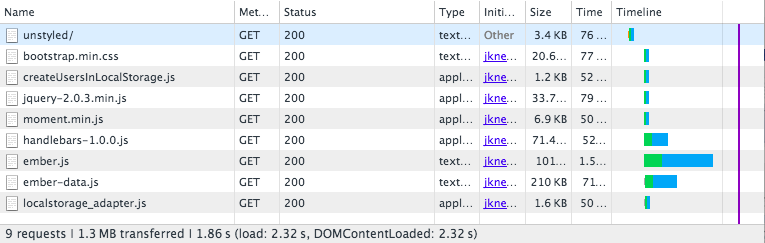
\includegraphics[width=0.8\textwidth]{images/performance_1.png}
    \caption{Übertragungszeit der benötigten Dateien}
    \label{fig:awesome_image}
\end{figure}
\begin{figure}[H]
    \centering
    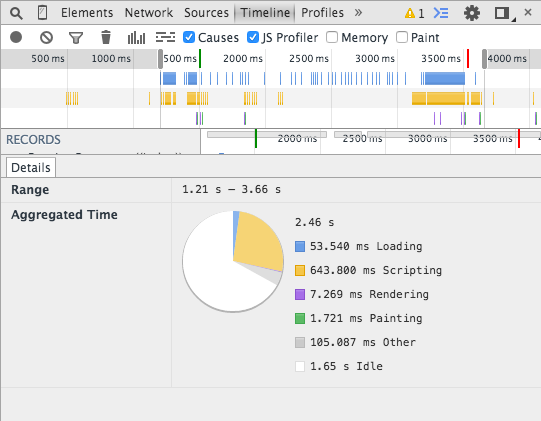
\includegraphics[width=0.6\textwidth]{images/performance_2.png}
    \caption{Benötigte Ausführungszeit der Skriptdatein}
    \label{fig:awesome_image}
\end{figure}
Die Ergebnisse zeigen, dass ganze $1.86s$ zum Übertragen und etwa $600ms$ zum ausführen den Anwendung benötigt wurden.

Aufgrund dessen wurde neben dem Versuch möglichst wenige Bibliotheken oder Frameworks zu benutzen (z.B. wenn nur eine Funktion einer großen Bibliothek benutzt wurde, wurde diese Funktion durch eine minimalere Bibliothek ersetzt oder selbst geschrieben bzw. kopiert.) auch diverse Techniken zum minimieren des Quelltextes genutzt.



\subsection*{Facebook React und die Flux Architektur}

Facebooks React\footnote{\url{https://github.com/facebook/react}} ist eine JavaScript-Bibliothek die seit ihrem erscheinen im Jahr 2013 viel Beifall und viele Anhänger finden konnte. Zum Zeitpunkt dieser Arbeit wird sie produktiv von vielen Firmen benutzt wie \textit{Khan Academy\footnote{\url{http://joelburget.com/backbone-to-react/}}}, \textit{Netflix\footnote{\url{http://conf.reactjs.com/schedule.html\#beyond-the-dom-how-netflix-plans-to-enhance-your-television-experience}}}, \textit{Yahoo!\footnote{\url{http://www.slideshare.net/mobile/rmsguhan/react-meetup-mailonreact}}}, \textit{Sony\footnote{\url{https://medium.com/code-stories/dev-chats-spike-brehm-of-airbnb-87e155f3475d}}} und anderen. Facebook benutzt sie selbst für ihre größten Produkte Facebook und Instagram (\textit{Google} benutzt ihr Framework \textit{AngularJS} z.B. nicht für das Flagschiff \textit{Google Mail}).

React ist jedoch kein Framework wie AngularJS oder Ember, es gibt keine Directives, Controllers, Templates oder Models. Das einzige was React bietet sind \textit{Components}, welche ähnlich wie der kommende Standard der \textit{Web Components}\footnote{\url{https://developer.mozilla.org/en-US/docs/Web/Web_Components}} wiederverwendbare Interface-Widgets darstellen indem Sie HTML/CSS und JavaScript koppeln und vom Rest des System separieren.

Dabei folgt React nicht den \textit{best-practices} die in den letzten Jahren in Webentwicklung entstanden sind und sich in MVC-Frameworks widerspiegeln. Klassisch gibt es ein Template, dass in HTML oder einem ähnlichen Sprache wie YAML geschrieben ist und Platzhalter enthält die später gefüllt werden - dies ist das V in MVC.
Dazu kommt ein Controller der diese Templates mit Daten füllt, auf welche Art ist nicht relevant. Kommuniziert der Controller mit einem Server um Daten zu übertragen wie die eines Benutzers stellt dies das M da, also nicht die Kommunikation selbst sondern die Datenstrukturen auf beiden Seiten die den Benutzer darstellen.
Applikationen auf diese Weise zu erstellen hat sich bewährt was jedoch nicht heißt es gibt keine Kritik.

\subsubsection*{Virtual DOM}

Wie weit muss ich hier den DOM beschreiben? Muss ich ihn beschreiben?

Einer der innovativsten Aspekte von React ist die virtuelle Repräsentation des DOMs\footnote{\url{http://de.wikipedia.org/wiki/Document_Object_Model}}. Die normale Interaktion mit dem DOM ist langsam und kompliziert, es ist sehr schwer den aktuellen Status der Applikation darüber abzubilden - so geschieht das häufig über CSS-Klassen oder speziellen Attributen.
Eine Lösung dieses Problems ist es die Applikation so zu schreiben, dass der ganze DOM bei jeder Veränderung des Zustands neu gerendert wird. (Vergleich hier zu Server-seitigem Rendern wo genau dies gemacht wird.) Natürlich wäre die Applikation bei so einem Vorgehen langsam (wegen des rendern durch den Browser) und Dinge wie Fokus auf Eingabe-Feldern würde verloren gehen was der Benutzer nicht gerade angenehm finden würde.

Mittels eines virtuellen DOMs kann dies deutlich effizienter und Benutzerfreundlicher gestaltet werden. Bei jeder Zustandsänderung wird ein neuer virtueller DOM erstellt und mit dem alten virtuellen verglichen wodurch die minimalen Änderungen erfasst werden können um den derzeitigen DOM zum Zustand des neuen zu bringen. Dies macht Frameworks die einen virtual DOM benutzen deutlich schneller als welche die die Hauptarbeit auf dem richtigen DOM verrichten. Das ganze Konzept ist skalierbar im Gegensatz zu Technologien wie dem \textit{dirty checking} von AngularJS welches eine Komplexität von $O(n^2)$ bis $O(n^10)$ (Ab 10 Iterationen wird abgebrochen) besitzt, wobei $n$ die Anzahl der veränderbaren Inhalte ist.
Der von Facebook verwendete Algorithmus besitzt eine Komplexität von $O(n)$\footnote{\url{https://facebook.github.io/react/docs/reconciliation.html}} wobei $n$ die Anzahl der DOM-Element ist.
Ein Geschwindikeitsvergleich von Frameworks die einen virtuellen DOM benutzen zeigt diese Grafik vom Elm\footnote{\url{http://en.wikipedia.org/wiki/Elm_programming_language}}-Entwickler bei der die verschiedenen Frameworks anhand ihrer TodoMVC\footnote{Der TodoMVC ist ein Versuch die schiere Anzahl an Webframeworks anhand eines realen Beispiels zu vergleichen. \url{http://todomvc.com/}}-Implementierung verglichen werden.

\begin{figure}[H]
    \centering
    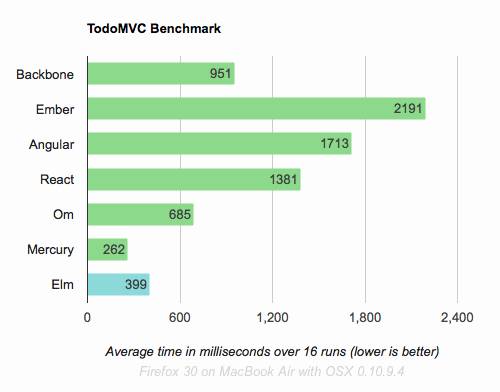
\includegraphics[width=1.0\textwidth]{images/virtual_dom.png}
    \caption{Geschwindigkeitsvergleich von TodoMVC-Implentierungen mit verschiedenen Frameworks.}
    \label{fig:awesome_image}
\end{figure}

Es ist zu sehen, dass Ember und AngularJS am langsamsten sind. Backbone ist in diesem Benchmark schneller als React, wobei die verwendete Implemtierung der React-App nicht optimiert ist - \textit{Om}\footnote{\url{https://github.com/omcljs/om}} kann als optimierte React-Version betrachtet werden, da Om im Grunde React mit nicht veränderbaren Datenstrukturen\footnote{Durch nicht veränderbare Datenstrukturen kann das diffing noch effizienter gestaltet werden, da viele Teilbäume nicht betrachtet werden müssen.} (immutable data-structures) ist. Backbone wie aber auch JQuery oder Dojo können theoretisch so schnell gemacht werden wie es möglich ist, dies ist aber so komplex, dass es nie gemacht wird und Wartbarkeit und Fehlervermeidung über Performance gestellt wird.
Die beiden schnellsten Frameworks benutzen ebenso eine virtual-DOM Implementierung und wie \textit{Om} auch nicht veränderbare Datenstrukturen.


Ein weiterer Vorteil der virtuellen Darstellung ist die Unabhängigkeit des Browsers um die Applikation zu rendern, dass schlussendliche rendern des virtuellen DOMs in den richtigen DOM ist nicht zwingend. Es ist z.B. möglich den virtuellen DOM in ein Canvas-Element zu rendern\footnote{\url{https://github.com/Flipboard/react-canvas}} oder ganz einfach in einen String. Durch das simple rendern zum String, was ganz ohne Browser möglich ist, beherrscht React isomorphes Rendering, d.h. die Inhalte können auf dem Server und im Client gerendert werden. So wird z.B. bei Instagram der erste Seitenaufruf auf dem Server alles weitere vom Clienten gerendert. Erste Versuche zeigen auch, dass man dies komplett agnostisch machen kann und alles kann auf Server/Client gerendert werden ohne das der Benutzer einen Unterschied merkt. So ist es denkbar das schwache Geräte mehr auf dem Server rendern und somit komplexe Inhalte vergleichsweise schnell darstellen können.

\subsubsection*{Flux Architektur}

Flux\footnote{\url{https://facebook.github.io/flux/docs/overview.html}} ist die Applikations-Architektur die Facebook für ihre Frontend-Applikationen benutzt, es ergänzt React insoweit dass es einen unidirektionellen Datenfluss ermöglicht. Es ist wie eine alternative zu MVC zu verstehen und ist mehr ein Muster um Applikationen zu schreiben als ein Framework das einem rigoros die Struktur vorschreibt. Im Allgemeinen benutzt Flux das Paradigma der Datenfluss Programierung\footnote{\url{http://en.wikipedia.org/wiki/Dataflow_programming}}, bei welchem ein Programm als gerichter Graph modelliert wird. Typisch für das Paradigma ist die Benutzung eines Beobachter-Entwursfmuster\footnote{\url{http://en.wikipedia.org/wiki/Observer_pattern}} wie z.B. eines pub/sub-System\footnote{Eine kleine Auflistung und eine Bewertung typischer Muster ist hier zu finden \url{https://github.com/millermedeiros/js-signals/wiki/Comparison-between-different-Observer-Pattern-implementations}}. Bei Flux wird für letzteres eine Abwandlung eines pub/sub-Systems benutzt.

Flux besitzt drei große Bestandteile: \textit{dispatcher}, \textit{stores}, \textit{views (React components)}. Desweiteren gibt es \textit{actions}, dies sind Hilfsmethoden vom \textit{dispatcher} und werden benutzt um eine semantische API zu unterstützen die alle Veränderungen die möglich sind in der Applikation beschreibt.

Das wichtigste Designziel von Flux ist der unidirektionale Datenfluss, wodurch die Logik deutlich verständlicher und nachvollziehbar wird.

\begin{figure}[H]
    \centering
    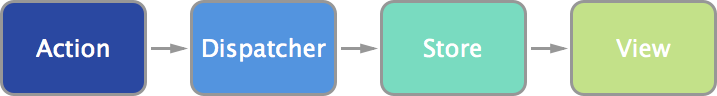
\includegraphics[width=1.0\textwidth]{images/flux.png}
    \caption{Dispatcher, Stores und Wiews sind unabhängige Knoten mit unterschiedlichen Ein und Ausgaben. Die Aktionen sind einfache Objekte die die neuen Daten enthalten und den Typ der Daten.}
    \label{fig:awesome_image}
\end{figure}

Diesem Schaubild zufolge ist es jedoch unmöglich dass eine \textit{Component} den Zustand der Applikation verändern kann, was jedoch so gut wie immer nötig ist. Hier für werden die \textit{actions} benutzt, diese können von den \textit{Components} benutzte werden um neue Daten an den Dispatcher zu schicken, welcher diese dann an den Store weiterleitet - welche dann die Darstellung der \textit{Component} beeinflussen kann.

\begin{figure}[H]
    \centering
    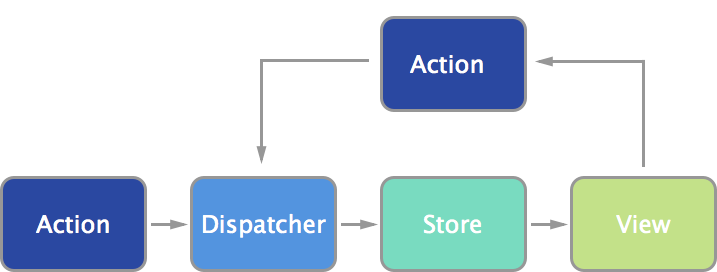
\includegraphics[width=1.0\textwidth]{images/flux_actions.png}
    \caption{Mithilfe von \textit{actions} ist die View in der Lage den Zustand der Applikation zu verändern.}
    \label{fig:awesome_image}
\end{figure}

Allem in allem ist die Facebook-Flux Architektur in Kombination mit React ein äußerst fortschrittlicher und zukunftssicherer Weg eine Webapplikation zu schreiben, womit die Anwendung dieser für die Erstellung der Enterprise-Wall eine gute Wahl erscheint.

\section*{Architektur der Applikation}

Wie im vorherigen Abschnitt beschrieben wurde mittels React und der Flux-Architektur realisiert. Anstelle der Flux-Bibliothek von Facebook wurde jedoch \textit{reflux} benutzt, \textit{reflux} vereinfacht Flux insofern als das es keinen einzelnen Dispatcher benutzte, jede Action ist ihr eigener Dispatcher mit dem Ziel Flux eben mehr zu vereinfachen und unnötigen Quelltext (sogennanten Boilerplate) zu reduzieren. Eine Vollständige Erklärung für \textit{reflux} ist auf dem Blog des Autors zu finden\footnote{\url{http://spoike.ghost.io/deconstructing-reactjss-flux/}}. \textit{reflux} ist nicht der einzige Versuch eine alternative bereitzustellen, mittlerweile gibt es über 10 verschiedene Flux-Bibliotheken\footnote{Ein Vergleich dieser ist hier zu finden \url{https://github.com/voronianski/flux-comparison}} - mit teilweise großen Communities dahinter oder Firmen wie z.B. \textit{Fluxible} von \textit{Yahoo}. Der Funktionsinhalt der verschiedenen Flux-Bibliotheken ist mehr oder minder gleich, somit könnte \textit{reflux} mit Leichtigkeit ausgetauscht werden, wenn es denn nötig wäre.

\subsection*{Überblick}

\begin{figure}[H]
    \centering
    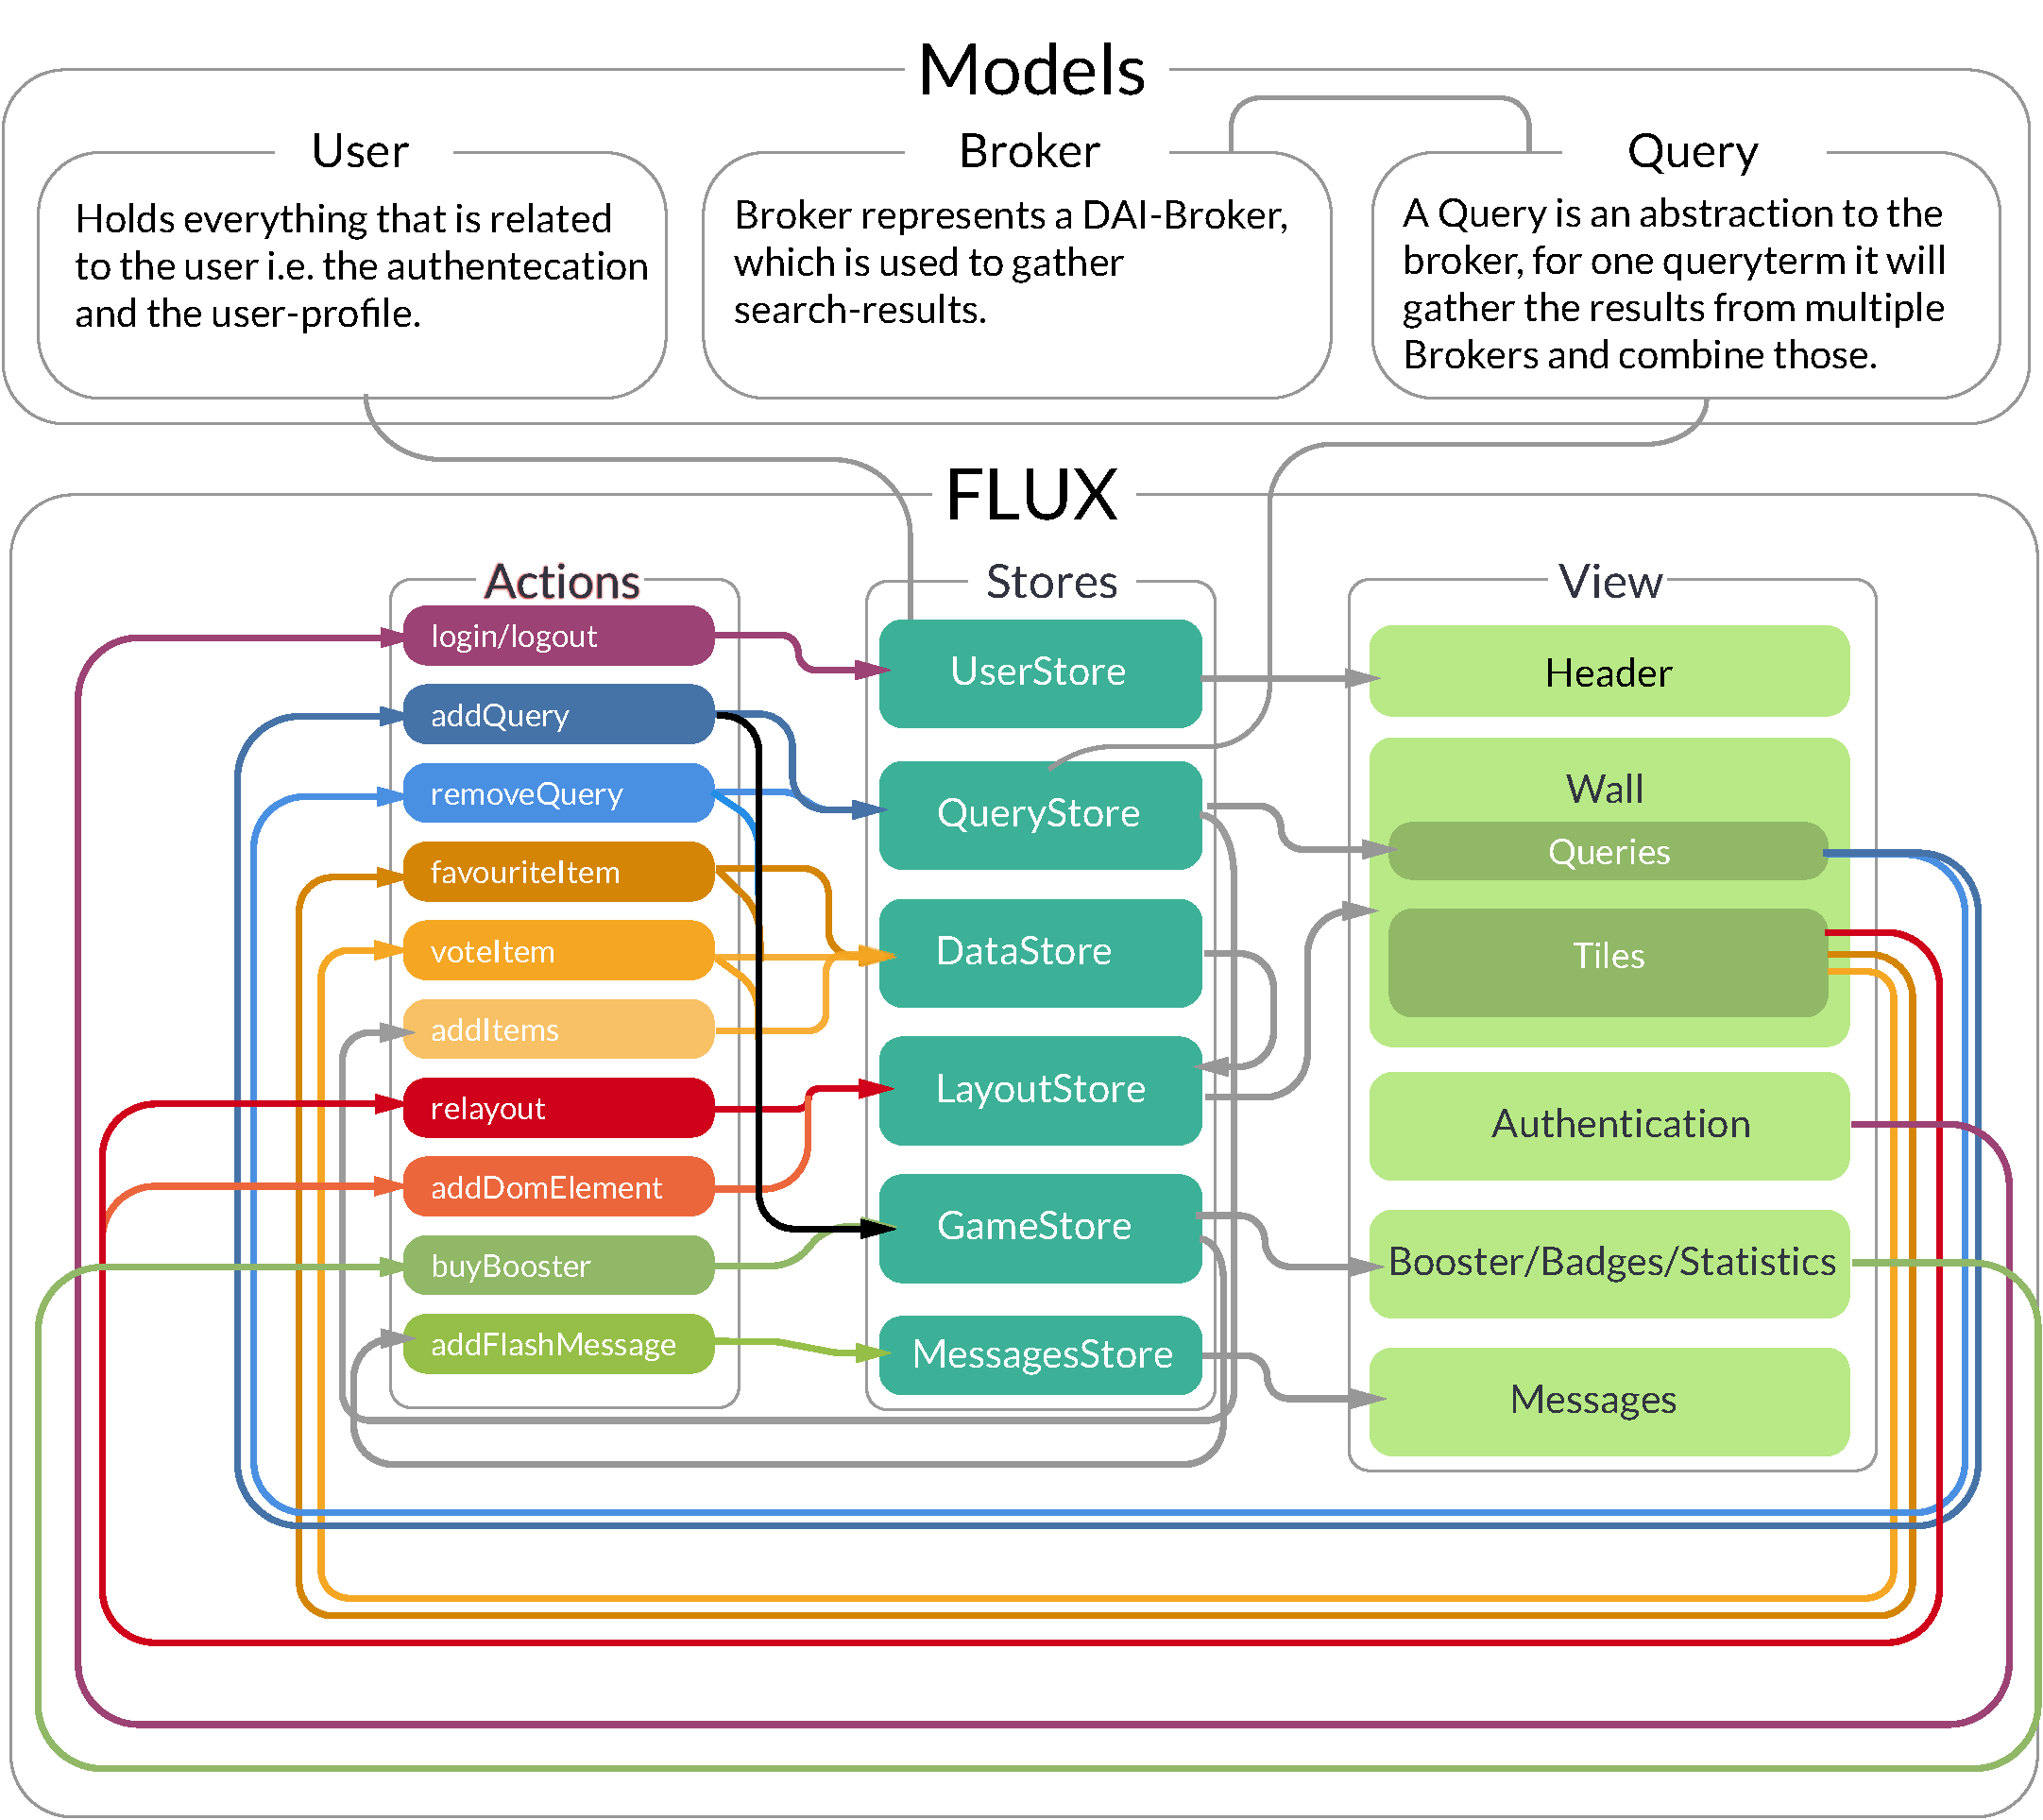
\includegraphics[width=1.0\textwidth]{images/architecture.pdf}
    \caption{Die wichtigsten Bestandteile der Applikation.}
    \label{fig:awesome_image}
\end{figure}

Die Architektur wurde bewusst nicht in einem Klassendiagramm dargestellt da die Applikation keinen Strengen Objektorienterten Stil verfolgt und das Schaubild nicht sonderlich zum Verständnis beitragen würde. Es ist auch kein komplettes Schaubild der Applikation, jegliche Aspekte die zum Verständnis nicht sonderlich beitragen würden wurden rausgelassen.

Wie zu sehen kann die Applikation in drei Teile eingeteilt werden.

\begin{enumerate}
  \item \textbf{Agenten} \\
  Die Agenten stellen die Kommunikation mit den jeweiligen Brokern da, sie implementieren alle eine Funktion \texttt{getData} die eine Suchanfrage  nimmt und eine einheitliche Datenstruktur mit den Ergebnissen zurückliefert. Broker die eine Authentifizierung benötigen liefern einen Fehler sobald so Benutzer-Objekt mit gültigen Token benutzt werden.
  \item \textbf{User - Authentifizierung}
  Der User beinhaltet neben seines Profils in welchem Favoriten, Punktestand und bewertete Suchergebnisse gespeichert werden die komplette Authentifizierung im System. Im aktuellen Zustand wird jeder Nutzer gezwungen sich zu authentifizieren um das System zu nutzen.
  \item \textbf{Flux - Actions, Stores und View}
  Dies ist der wichtigste, komplizierteste und größte Teil der Applikation. Hier geschieht alles was mit dem Darstellen und der Interaktion mit den Inhalten zu tun hat. In den Stores werden die Daten der Agenten soweit verarbeitet dass sie an die View weitergegeben können wo sie als interaktive Kacheln dargestellt werden. Interaktionen geschehen über die Aktionen. Es ist gut zu sehen dass der Datenfluss Unidirektionell ist, wodurch das urteilen über Applikation vereinfacht wird.

\end{enumerate}

Im folgenden werde ich genauer auf den Flux-Teil eingehen.

\subsection*{Stores - Data}

Der DataStore stellt alle Daten bereit die für die Darstellung benötigt werden, dies sind die Suchergbnisse die mit dem Profil des Benutzers gemixt werden um anzuzeigen welche Ergebnisse bewertet/favorisiert wurden und die Suchanfragen, die zur Laufzeit verändert werden können. Herausforderungen hier waren es Duplikate in den Suchergebnissen auszuschließen, Anfragen an die Broker zu minimieren und die Interaktion mit den Suchergebnissen.

Eine Besonderheit ist die Benutzung einer nicht veränderbaren OrderedMap in welcher die Suchergbnisse mit ihrer \textit{url} als Schlüssel gespeichert sind. Die Suchergbnisse werden in der Applikation noch viel weitergereicht weswegen viele Fehler vorgebeugt werden da nur der DataStore selbst die Suchergebnisse verändern kann.

\subsection*{Stores - Layout}

Im Design-Abschnitt wurde lange darauf eingegangen was die Layouting-Engine alles können muss, leider konnte keine der OpenSource-Bibliotheken allen Anforderungen gerecht werden. Deswegen wurde extra für die Darstellung eine eigene Layouting-Engine erstellt.
Die Grundlage ist die absolute Positionierung innerhalb des Browsers, diese ist notwendig um Animationen zu ermöglichen. Es gibt verschiedene Arten DOM-Elemente mittels css zu positionieren:

\begin{enumerate}
  \item Mithilfe von \texttt{top/left}.\\
  \begin{minted}{css}
  .position-top-left {
      position: absolute; /* or relative/fixed */
      top:  50px;
      left: 50px;
  }
  \end{minted}
  \item Mithilfe von \texttt{transform: translate(x, y)}. Dies ist allgemein anerkannt schneller als zu sein und hat den Vorteil das subpixel-animationen möglich sind was im Allgemeinen flüssigere Animationen erlaubt. \\
  \begin{minted}{css}
  .position-translate {
      position: absolute; /* or relative/fixed */
      transform:         translate(50px, 50px);
      -webkit-transform: translate(50px, 50px);
  }
  \end{minted}
  \item Mithilfe von \texttt{transform: translate3D(x, y, z)}. Dies ist mit Abstand das schnellste. Hierbei werden die Elemente zu Texturen gerendert und mit Einsatz des Grafikprozessors animiert. Dadurch ist es sogar möglich auf mobilen Endgeräten flüssige Animationen zu haben, da diese meist dedidizierte Grafikprozessoren haben.
  \begin{minted}{css}
  .position-translate3D {
      position: absolute; /* or relative/fixed */
      transform:         translate3D(50px, 50px);
      -webkit-transform: translate3D(50px, 50px);
  }
  \end{minted}
  \texttt{transform3D} wird von allen aktuellen Browsern soweit unterstützt das unser Szenario möglich ist\footnote{\url{http://caniuse.com/\#feat=transforms3d}}. Was weiterhin zu beachten ist, dass am Ende immer gerundete Pixelwerte innerhalb von \textsc{translate3D(x, y, z)} benutzt werden sollten. Da Ansonsten die Elemente unscharf sind.

\end{enumerate}

Es ist eine Grundanforderung Geräte mit unterschiedlich Großen Bildschirmen zu unterstützen, was dadurch erzielt wird, dass die die Anzahl der Spalten variabel ist.
Es gibt zwei Möglichkeiten die Anzahl der Spalten variabel zu machen:

\begin{enumerate}
  \item Berechne die Breite mittels Javascript bevor das Element in den DOM eingefügt wird und setze die Breite mittels css.
  \item Durch die Benutzung von \textit{Media Queries} können in css verschiedene Darstellungen für unterschiedliche Bildschrimbreiten beschrieben werden. 
\end{enumerate}

Für die Positionierung müssen wir wissen wieviel Spalten zu jedem Zeitpunkt dargestellt werden sollen. Dafür muss die Breite in Javascript berechnet werden, somit liegt 1. nahe. Versuche haben jedoch gezeigt, dass es schneller ist die Breite des Elementes nicht per Javascript zu setzen sondern diese über die Media-Queries zu bestimmen. Zwar bedeuted dies, dass die gleiche Logik an zwei Orten in 2 Sprachen steht, aber da dies nicht mehr als jeweils 10 Zeilen sind ist es für die resultierende bessere Geschwindigkeit hinnehmbar.

Die Breite aller Elemente ist zu jedem Zeitpunkt gleich, die Höhe ist jedoch variabel. Da es unmöglich ist die Höhe auszurechnen ohne eine komplette Browser-Engine zu implementieren, muss das Element in den DOM eingefügt werden bevor wir dessen korrekte y-Position berechnen können.


\section*{Backend}

Im Verlaufe der Arbeit wurde entschieden, dass eine weitere Server-Applikation ungünstig wäre und die Arbeiten im Frontend ausreichend waren für den Rahmen einer Bachelor-Arbeit.
Zur Vollständigkeit halber werden die verwendeten Technologien aufgezählt.


\chapter{Ausblick}

\chapter{Appendix}

\cleardoublepage
\phantomsection

\printbibliography

\cleardoublepage
\phantomsection

\end{document}
